%% 由 build/emit_tex.py 生成（生成物，勿手改）；定制请放 user_style.tex / user_meta.yaml
\chapter{第 9 章 · AI Agent
编程基础}\label{ux7b2c-9-ux7ae0-ai-agent-ux7f16ux7a0bux57faux7840}

\section{01 AI 编程与 Agent
基础}\label{ai-ux7f16ux7a0bux4e0e-agent-ux57faux7840}

\begin{quote}
本节回答三个问题：Agent 编程与''AI 帮我写代码''到底差在哪？一个 Agent
内部做了什么？哪些事必须自己管？ 阅读约 25 分钟；配套图 4
张，可直接运行的代码 1 段。
\end{quote}

\subsection{本节目标}\label{ux672cux8282ux76eeux6807-31}

\begin{enumerate}
\def\labelenumi{\arabic{enumi}.}
\tightlist
\item
  说清\textbf{代码补全、对话式编程、Agent
  编程}三者的差别，并解释''闭环''为什么是关键。
\item
  用\textbf{五件套}描述一个 agent
  harness（智能体框架）：模型、工具、上下文、权限、会话。
\item
  复述\textbf{一次 Agent 循环}的五个动作，并能把一个小任务拆成循环。
\item
  解释\textbf{上下文窗口与压缩}，知道怎么''省上下文''。
\item
  说出\textbf{权限三档}与审批机制，记住数据红线在哪里。
\item
  识别\textbf{四种典型失败模式}，并给出至少一条对策。
\end{enumerate}

\subsection{先修}\label{ux5148ux4fee-24}

\begin{itemize}
\tightlist
\item
  完成第 0 章的环境安装：会用终端（PowerShell / Bash）、会运行 python
  脚本；
\item
  学完第 1 章 NumPy：本节的演示案例用到 axis 与广播；
\item
  不需要任何机器学习或大模型背景。
\end{itemize}

\subsection{术语速查（中英对照）}\label{ux672fux8bedux901fux67e5ux4e2dux82f1ux5bf9ux7167}

后续章节会反复用到这些词，先混个脸熟即可：

{\def\LTcaptype{none} % do not increment counter
\begin{longtable}[]{@{}
  >{\raggedright\arraybackslash}p{(\linewidth - 4\tabcolsep) * \real{0.3333}}
  >{\raggedright\arraybackslash}p{(\linewidth - 4\tabcolsep) * \real{0.3333}}
  >{\raggedright\arraybackslash}p{(\linewidth - 4\tabcolsep) * \real{0.3333}}@{}}
\toprule\noalign{}
\begin{minipage}[b]{\linewidth}\raggedright
术语
\end{minipage} & \begin{minipage}[b]{\linewidth}\raggedright
英文
\end{minipage} & \begin{minipage}[b]{\linewidth}\raggedright
一句话解释
\end{minipage} \\
\midrule\noalign{}
\endhead
\bottomrule\noalign{}
\endlastfoot
智能体 & Agent & 能自己调用工具、执行多步任务来完成目标的 AI 程序 \\
智能体框架 & Agent harness &
把模型、工具、上下文、权限、会话组装起来跑循环的软件 \\
工具调用 & Tool call &
模型请求执行一个动作（读文件、跑命令、搜索）并拿到结果 \\
上下文 & Context &
模型这一次能看到的全部内容：指令、历史、文件片段、工具输出 \\
压缩 & Compaction & 上下文快满时，把过程压缩成''目标 + 结论 + 证据'' \\
权限 & Permission & 决定 Agent 能做什么、哪些动作需要你点头 \\
沙箱 & Sandbox & 限制 Agent 只能访问指定范围的机制 \\
技能 & Skill & 预先写好的领域工作流，按需加载进上下文 \\
子代理 & Subagent & 由主代理派生、专门做一件事的独立 Agent \\
计划模式 & Plan mode & 先产出计划、经你确认后再动手的工作方式 \\
会话 & Session & 一次持续的对话上下文，可保存、继续、回看 \\
工作区 & Workspace & Agent 默认能读写的项目目录 \\
\end{longtable}
}

\subsection{正文}\label{ux6b63ux6587-3}

\subsubsection{1.
三代编程助手：从''猜下一行''到''自己动手''}\label{ux4e09ux4ee3ux7f16ux7a0bux52a9ux624bux4eceux731cux4e0bux4e00ux884cux5230ux81eaux5df1ux52a8ux624b}

\begin{figure}
\centering
\pandocbounded{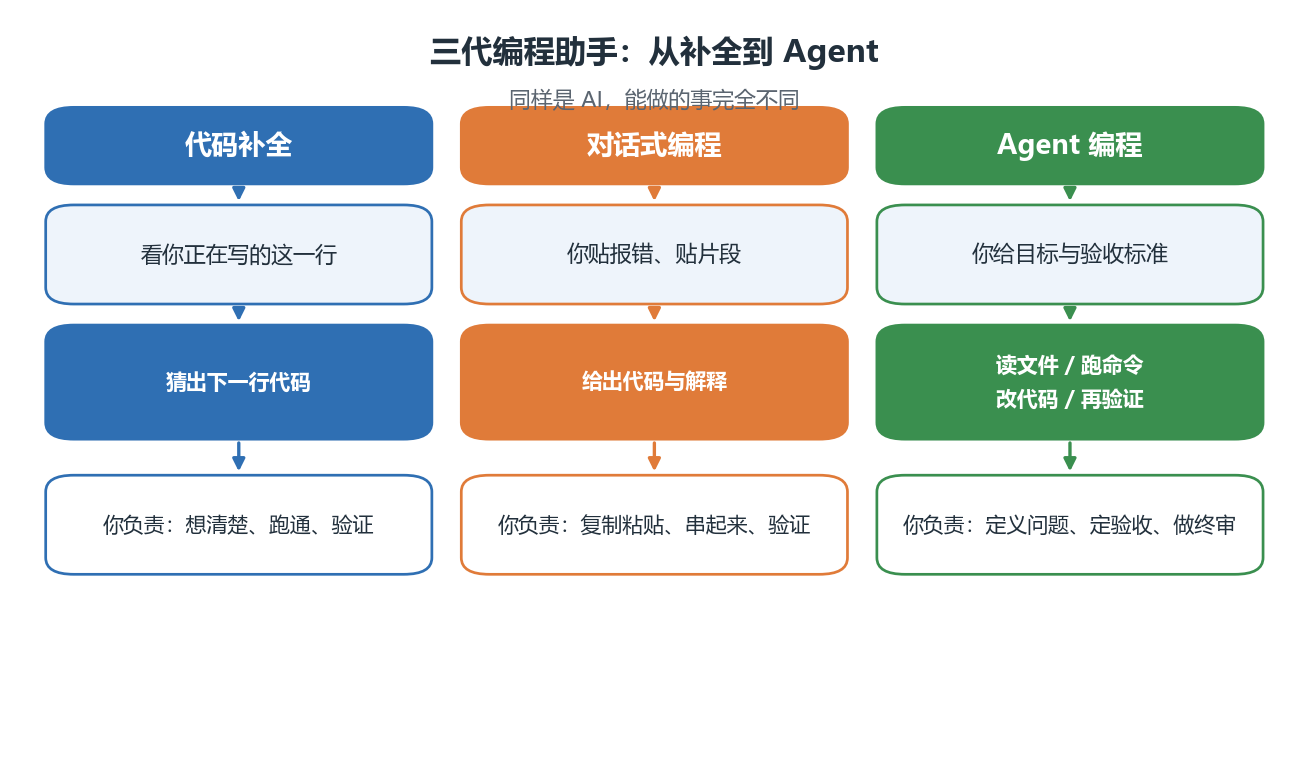
\includegraphics[keepaspectratio,alt={三代编程助手对比}]{figures/09-agent-basics/agent_vs_completion.png}}
\caption{三代编程助手对比}
\end{figure}

{\def\LTcaptype{none} % do not increment counter
\begin{longtable}[]{@{}
  >{\raggedright\arraybackslash}p{(\linewidth - 6\tabcolsep) * \real{0.2500}}
  >{\raggedright\arraybackslash}p{(\linewidth - 6\tabcolsep) * \real{0.2500}}
  >{\raggedright\arraybackslash}p{(\linewidth - 6\tabcolsep) * \real{0.2500}}
  >{\raggedright\arraybackslash}p{(\linewidth - 6\tabcolsep) * \real{0.2500}}@{}}
\toprule\noalign{}
\begin{minipage}[b]{\linewidth}\raggedright
\end{minipage} & \begin{minipage}[b]{\linewidth}\raggedright
代码补全
\end{minipage} & \begin{minipage}[b]{\linewidth}\raggedright
对话式编程
\end{minipage} & \begin{minipage}[b]{\linewidth}\raggedright
Agent 编程
\end{minipage} \\
\midrule\noalign{}
\endhead
\bottomrule\noalign{}
\endlastfoot
你给它 & 正在写的这一行 & 报错、代码片段、问题 & 目标 + 约束 +
\textbf{验收标准} \\
它给你 & 猜出的下一行 & 代码与解释 &
读文件、跑命令、改代码、再验证的\textbf{完整过程} \\
你负责 & 想清楚、跑通、验证 & 复制粘贴、串起来、验证 &
定义问题、定验收、做终审 \\
出错时 & 你改 & 你改 & 它自己看报错再改（直到你设的验收标准满足） \\
\end{longtable}
}

三者的分水岭是\textbf{闭环}：前两代的输出是''文本''，你拿到文本后还要自己去运行、观察、判断、再回来描述问题；Agent
的输出是''完成的动作''------它有眼睛（读文件、看报错）和手（改文件、跑命令），能在这个循环里自我修正。

一句话记住：\textbf{补全帮你写一行，对话帮你写一段，Agent
帮你把事情做完------但''做对''的定义仍然由你给出。}

\subsubsection{2.
harness：模型之外的四件事}\label{harnessux6a21ux578bux4e4bux5916ux7684ux56dbux4ef6ux4e8b}

\begin{figure}
\centering
\pandocbounded{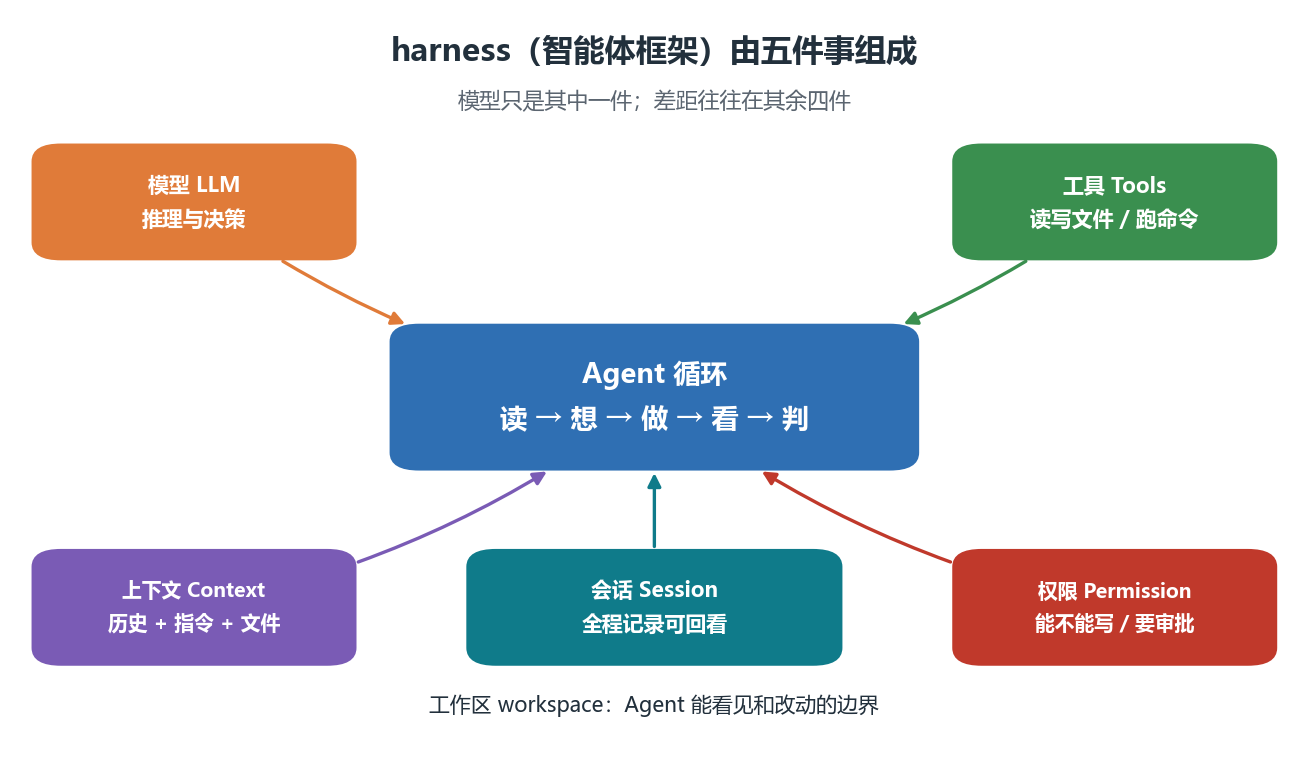
\includegraphics[keepaspectratio,alt={harness 的组成}]{figures/09-agent-basics/harness_anatomy.png}}
\caption{harness 的组成}
\end{figure}

很多人以为''用了同一个模型，效果应该差不多''。实际上，同一个模型在不同
harness 里的表现可以差很远，因为决定体验的是另外四件事：

{\def\LTcaptype{none} % do not increment counter
\begin{longtable}[]{@{}
  >{\raggedright\arraybackslash}p{(\linewidth - 4\tabcolsep) * \real{0.3333}}
  >{\raggedright\arraybackslash}p{(\linewidth - 4\tabcolsep) * \real{0.3333}}
  >{\raggedright\arraybackslash}p{(\linewidth - 4\tabcolsep) * \real{0.3333}}@{}}
\toprule\noalign{}
\begin{minipage}[b]{\linewidth}\raggedright
组成
\end{minipage} & \begin{minipage}[b]{\linewidth}\raggedright
作用
\end{minipage} & \begin{minipage}[b]{\linewidth}\raggedright
少了它会怎样
\end{minipage} \\
\midrule\noalign{}
\endhead
\bottomrule\noalign{}
\endlastfoot
模型 LLM & 推理与决策 & 没有大脑，什么也做不了 \\
工具 Tools & 读写文件、跑命令、搜索 & 只能说不能做，等于聊天机器人 \\
上下文 Context & 把项目指令、历史、文件内容喂给模型 &
它不知道你的项目规范，反复问同样的问题 \\
权限 Permission & 决定能不能写、要不要审批 &
要么什么都不敢做，要么风险失控 \\
会话 Session & 记录全部动作，可继续、可回看 &
每次从零开始，出了问题无法追责 \\
\end{longtable}
}

\begin{quote}
类比：模型是发动机，harness
是底盘、变速箱、刹车和仪表盘。发动机再好，没有刹车也不敢上路。
\end{quote}

\subsubsection{3. 一次 Agent
循环的解剖}\label{ux4e00ux6b21-agent-ux5faaux73afux7684ux89e3ux5256}

\begin{figure}
\centering
\pandocbounded{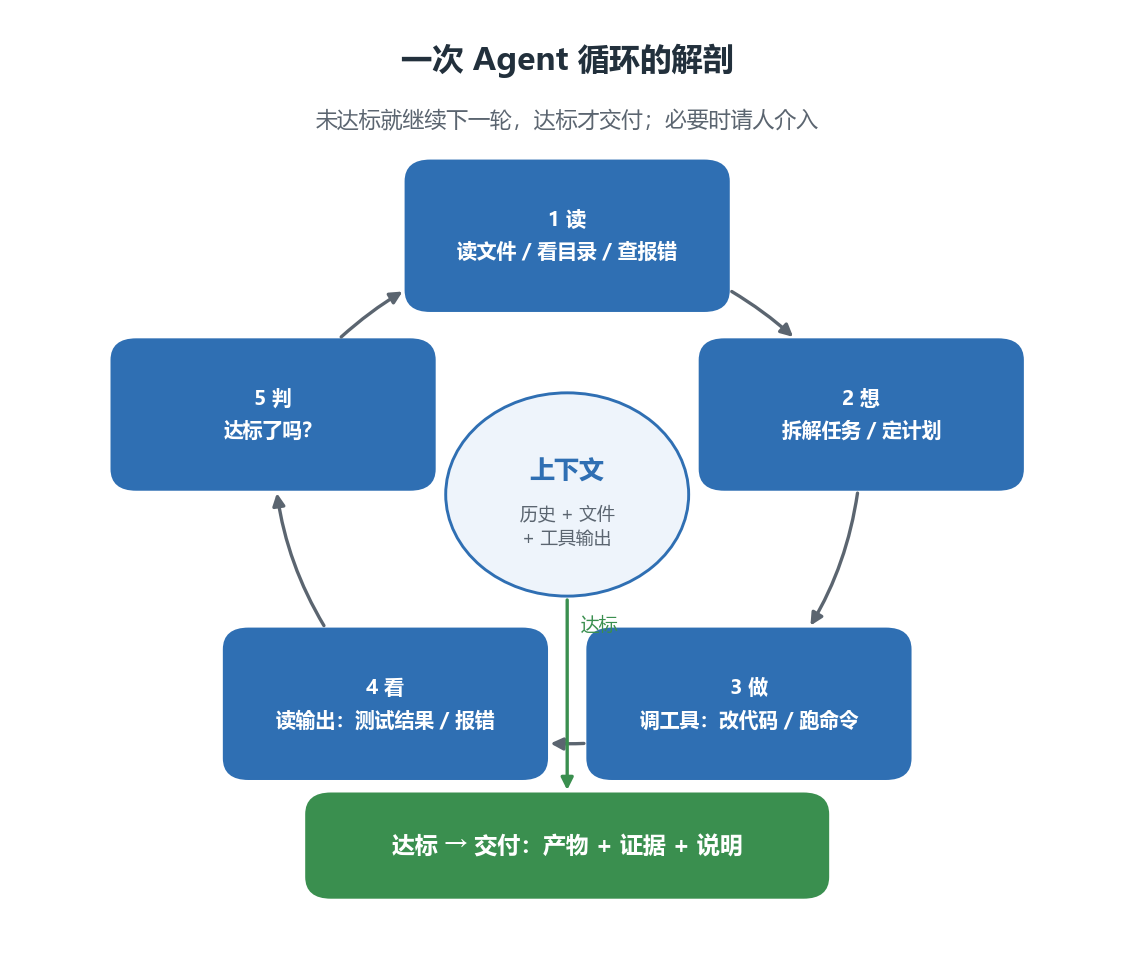
\includegraphics[keepaspectratio,alt={一次 Agent 循环}]{figures/09-agent-basics/agent_loop.png}}
\caption{一次 Agent 循环}
\end{figure}

循环只有五个动作，但每一步都有讲究：

\begin{enumerate}
\def\labelenumi{\arabic{enumi}.}
\tightlist
\item
  \textbf{读}：看目录、读文件、看报错。它看到什么，取决于你给的工作区与上下文。
\item
  \textbf{想}：拆解任务、定计划。复杂任务建议先进入\textbf{计划模式}，让你确认后再动手。
\item
  \textbf{做}：调用工具------改代码、跑脚本、装依赖、查文档。
\item
  \textbf{看}：读回执行结果。这一步是 Agent
  与''聊天''最大的区别：它必须面对真实输出。
\item
  \textbf{判}：达标了吗？达标的判据\textbf{不是''代码跑起来了''，而是你事先给的验收标准}。
\end{enumerate}

用一个具体任务走一遍。假设你有一份成绩矩阵，想算''每个学生的平均分''，但代码写成了按列求平均：

\begin{itemize}
\tightlist
\item
  读：Agent 打开脚本，看到 scores 的形状是 (4, 3)、代码里写着
  mean(axis=0)。
\item
  想：它需要判断你的\textbf{意图}------``每个学生''对应行还是列。
\item
  做：它写出最小复现，分别打印两种 axis 的结果和形状。
\item
  看：形状一个 (3,) 一个 (4,)，它意识到意图与实现不一致。
\item
  判：按你给的验收标准（形状必须是
  (4,)、数值与手算一致）给出结论与修复。
\end{itemize}

\begin{quote}
关键认识：\textbf{循环的终止条件由你定义。} 没有验收标准，Agent
就会以''看起来能跑''作为终点。
\end{quote}

\subsubsection{4. 上下文：Agent
的短期记忆}\label{ux4e0aux4e0bux6587agent-ux7684ux77edux671fux8bb0ux5fc6}

\begin{figure}
\centering
\pandocbounded{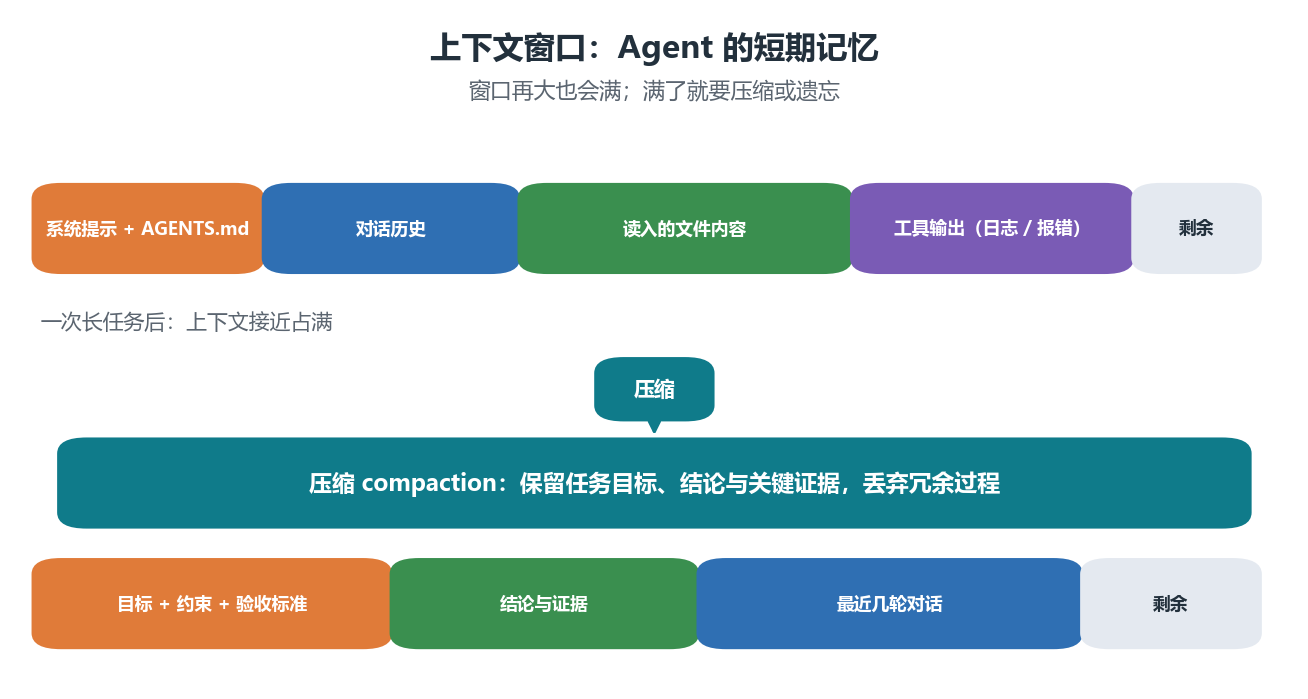
\includegraphics[keepaspectratio,alt={上下文窗口与压缩}]{figures/09-agent-basics/context_window.png}}
\caption{上下文窗口与压缩}
\end{figure}

上下文窗口再大也会满。一次长任务里，系统提示、对话历史、读入的文件、工具输出会迅速堆积；快满时
harness
会做\textbf{压缩（compaction）}，把过程浓缩成目标、结论与关键证据。

三条实用建议：

\begin{enumerate}
\def\labelenumi{\arabic{enumi}.}
\tightlist
\item
  \textbf{给最小可复现}：一段 20 行的复现脚本，比 2000
  行项目源码更有用。
\item
  \textbf{让它自己读文件}：说''读 src/clean.py 里 load\_data
  函数''比把代码整段贴进对话更省上下文，也更准确。
\item
  \textbf{长任务主动收口}：阶段结束时让它总结''已确认的结论 +
  未解决的问题 + 下一步''，这既是压缩，也是你检查方向的时机。
\end{enumerate}

\paragraph{案例卡 1：一个''看起来都对''的错误------axis
用反了}\label{ux6848ux4f8bux5361-1ux4e00ux4e2aux770bux8d77ux6765ux90fdux5bf9ux7684ux9519ux8befaxis-ux7528ux53cdux4e86}

\textbf{目标}：认识''静默数值错误''------代码能跑、数字看着合理，但结论是错的。

\textbf{代码}

\begin{Shaded}
\begin{Highlighting}[]
\ImportTok{import}\NormalTok{ numpy }\ImportTok{as}\NormalTok{ np}
\NormalTok{np.set\_printoptions(precision}\OperatorTok{=}\DecValTok{2}\NormalTok{, suppress}\OperatorTok{=}\VariableTok{True}\NormalTok{)}

\NormalTok{scores }\OperatorTok{=}\NormalTok{ np.array([[}\DecValTok{82}\NormalTok{, }\DecValTok{90}\NormalTok{, }\DecValTok{78}\NormalTok{],}
\NormalTok{                   [}\DecValTok{60}\NormalTok{, }\DecValTok{65}\NormalTok{, }\DecValTok{70}\NormalTok{],}
\NormalTok{                   [}\DecValTok{95}\NormalTok{, }\DecValTok{88}\NormalTok{, }\DecValTok{92}\NormalTok{],}
\NormalTok{                   [}\DecValTok{70}\NormalTok{, }\DecValTok{72}\NormalTok{, }\DecValTok{68}\NormalTok{]], dtype}\OperatorTok{=}\BuiltInTok{float}\NormalTok{)}

\NormalTok{by\_exam }\OperatorTok{=}\NormalTok{ scores.mean(axis}\OperatorTok{=}\DecValTok{0}\NormalTok{)}
\NormalTok{by\_student }\OperatorTok{=}\NormalTok{ scores.mean(axis}\OperatorTok{=}\DecValTok{1}\NormalTok{)}

\BuiltInTok{print}\NormalTok{(}\StringTok{"by\_exam   :"}\NormalTok{, by\_exam, }\StringTok{"shape"}\NormalTok{, by\_exam.shape)}
\BuiltInTok{print}\NormalTok{(}\StringTok{"by\_student:"}\NormalTok{, by\_student, }\StringTok{"shape"}\NormalTok{, by\_student.shape)}
\BuiltInTok{print}\NormalTok{(}\StringTok{"mean of all:"}\NormalTok{, }\BuiltInTok{round}\NormalTok{(}\BuiltInTok{float}\NormalTok{(scores.mean()), }\DecValTok{3}\NormalTok{))}
\BuiltInTok{print}\NormalTok{(}\StringTok{"sum check :"}\NormalTok{, }\BuiltInTok{round}\NormalTok{(}\BuiltInTok{float}\NormalTok{(by\_exam.}\BuiltInTok{sum}\NormalTok{()), }\DecValTok{3}\NormalTok{), }\BuiltInTok{round}\NormalTok{(}\BuiltInTok{float}\NormalTok{(by\_student.}\BuiltInTok{sum}\NormalTok{()), }\DecValTok{3}\NormalTok{))}
\end{Highlighting}
\end{Shaded}

\textbf{运行结果（已运行核验）}

\begin{Shaded}
\begin{Highlighting}[]
\NormalTok{by\_exam   : [76.75 78.75 77.  ] shape (3,)}
\NormalTok{by\_student: [83.33 65.   91.67 70.  ] shape (4,)}
\NormalTok{mean of all: 77.5}
\NormalTok{sum check : 232.5 310.0}
\end{Highlighting}
\end{Shaded}

\textbf{讲解}

\begin{itemize}
\tightlist
\item
  两个结果都是''合理的分数''，粗看都像平均分------这正是静默错误可怕的地方；
\item
  形状是第一个判据：想算''每个学生''就该得到 4 个数，得到 3
  个说明方向错了；
\item
  总和是第二个判据：by\_exam 的均值之和 232.5 只是总分 930
  的三分之一，by\_student 的 310.0 才是''每人平均分之和''；
\item
  只打印数字、不做判据检查，这类错误可以躲过一整天。
\end{itemize}

\textbf{主要用法 / API}

{\def\LTcaptype{none} % do not increment counter
\begin{longtable}[]{@{}ll@{}}
\toprule\noalign{}
用法 & 说明 \\
\midrule\noalign{}
\endhead
\bottomrule\noalign{}
\endlastfoot
array.mean(axis=k) & 沿第 k 维求平均：k=0 消掉行、k=1 消掉列 \\
array.shape & 判断结果方向是否符合意图的第一判据 \\
np.set\_printoptions & 控制打印精度，避免误以为''数不一样'' \\
\end{longtable}
}

\textbf{常见错误}

\begin{enumerate}
\def\labelenumi{\arabic{enumi}.}
\tightlist
\item
  只把结果打印出来看一眼''像不像''，不用形状与守恒量检查；
\item
  把 axis=0 记成''对每一行''（其实是沿行方向压缩，得到每列的值）；
\item
  让 Agent 修 bug
  时只说''结果不对''，不说\textbf{期望的形状与判据}，它只能猜。
\end{enumerate}

\textbf{拓展}

\begin{itemize}
\tightlist
\item
  把 scores 换成 (3, 4, 5) 的三维数组，先说出 mean(axis=1)
  的形状，再运行验证；
\item
  让 Agent 写一个 3 行的断言函数，把''形状必须是 (4,)``固化成测试；
\item
  思考：如果这份数据是某次实验的唯一结果，这个错误会怎样影响结论？
\end{itemize}

\subsubsection{5.
人机分工：什么交给它，什么必须自己管}\label{ux4ebaux673aux5206ux5de5ux4ec0ux4e48ux4ea4ux7ed9ux5b83ux4ec0ux4e48ux5fc5ux987bux81eaux5df1ux7ba1}

{\def\LTcaptype{none} % do not increment counter
\begin{longtable}[]{@{}lll@{}}
\toprule\noalign{}
任务类型 & 建议 & 原因 \\
\midrule\noalign{}
\endhead
\bottomrule\noalign{}
\endlastfoot
样板代码、格式转换、批量重命名 & 交给 Agent & 规则明确、易验证 \\
写测试、补边界条件、重构 & 交给 Agent（你审 diff） & 有客观判据 \\
查文档、读陌生代码库、写注释 & 交给 Agent & 信息检索型工作 \\
问题定义与建模 & \textbf{人主导} & 决定''做什么''，Agent 无法替你决定 \\
验收标准与数据判据 & \textbf{人主导} & 决定''什么叫做对'' \\
结论与解释 & \textbf{人主导}（Agent 只能起草） & 涉及因果、局限与责任 \\
\end{longtable}
}

三条铁律：\textbf{问题定义归人、验收标准归人、结论归人。} Agent
可以在这三件事上给建议，但不能替你签字。

\subsubsection{6. 权限与安全：让 Agent
在笼子里干活}\label{ux6743ux9650ux4e0eux5b89ux5168ux8ba9-agent-ux5728ux7b3cux5b50ux91ccux5e72ux6d3b}

\begin{figure}
\centering
\pandocbounded{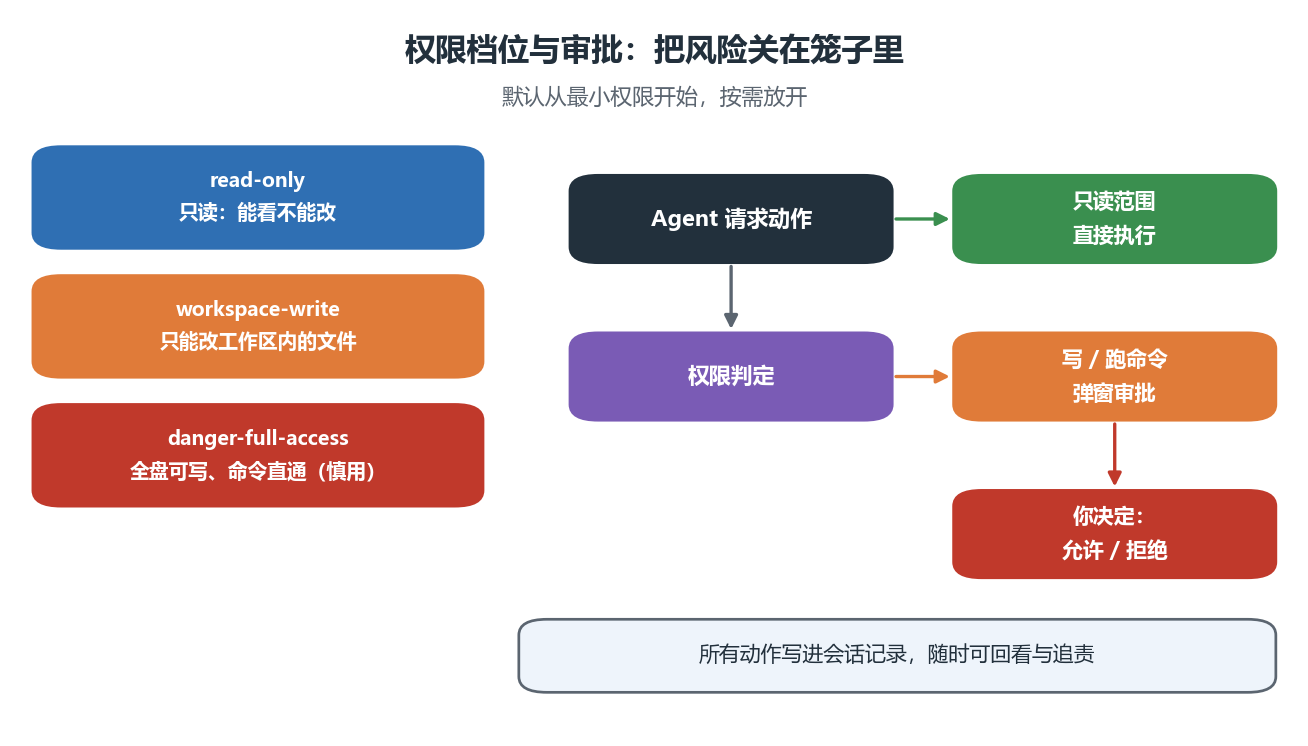
\includegraphics[keepaspectratio,alt={权限档位与审批}]{figures/09-agent-basics/permission_flow.png}}
\caption{权限档位与审批}
\end{figure}

主流 harness 都提供分档权限，常见三档：

{\def\LTcaptype{none} % do not increment counter
\begin{longtable}[]{@{}
  >{\raggedright\arraybackslash}p{(\linewidth - 4\tabcolsep) * \real{0.3333}}
  >{\raggedright\arraybackslash}p{(\linewidth - 4\tabcolsep) * \real{0.3333}}
  >{\raggedright\arraybackslash}p{(\linewidth - 4\tabcolsep) * \real{0.3333}}@{}}
\toprule\noalign{}
\begin{minipage}[b]{\linewidth}\raggedright
档位
\end{minipage} & \begin{minipage}[b]{\linewidth}\raggedright
含义
\end{minipage} & \begin{minipage}[b]{\linewidth}\raggedright
适用场景
\end{minipage} \\
\midrule\noalign{}
\endhead
\bottomrule\noalign{}
\endlastfoot
read-only & 只能读，不能改 & 第一次接触陌生项目、只想让它解释代码 \\
workspace-write & 只能改工作区内的文件 &
日常开发、课程作业（\textbf{推荐默认}） \\
danger-full-access & 全盘可写、命令直通 & 受控环境下的高级用法，慎用 \\
\end{longtable}
}

配套机制是\textbf{审批}：涉及写文件、跑命令、装依赖时，界面会先问你；你的每一次允许或拒绝都会写进会话记录，可回看、可追责。

数据红线（请直接记住）：

\begin{itemize}
\tightlist
\item
  不要把隐私数据（身份证、手机号、成绩单、医疗记录）贴进对话；
\item
  不要把涉密或未发表的数据交给云端模型；
\item
  不要把别人的 API Key、密码、令牌放进提示词或代码；
\item
  处理真实数据前，先想清楚''这份数据能不能离开这台机器''。
\end{itemize}

\subsubsection{7.
四种典型失败模式与对策}\label{ux56dbux79cdux5178ux578bux5931ux8d25ux6a21ux5f0fux4e0eux5bf9ux7b56}

{\def\LTcaptype{none} % do not increment counter
\begin{longtable}[]{@{}
  >{\raggedright\arraybackslash}p{(\linewidth - 4\tabcolsep) * \real{0.3333}}
  >{\raggedright\arraybackslash}p{(\linewidth - 4\tabcolsep) * \real{0.3333}}
  >{\raggedright\arraybackslash}p{(\linewidth - 4\tabcolsep) * \real{0.3333}}@{}}
\toprule\noalign{}
\begin{minipage}[b]{\linewidth}\raggedright
失败模式
\end{minipage} & \begin{minipage}[b]{\linewidth}\raggedright
长什么样
\end{minipage} & \begin{minipage}[b]{\linewidth}\raggedright
对策
\end{minipage} \\
\midrule\noalign{}
\endhead
\bottomrule\noalign{}
\endlastfoot
幻觉 API & 编出不存在的函数、参数、配置项 &
要求它运行验证；自己查一眼官方文档 \\
静默数值错误 & 能跑、数字合理，其实方向或单位错了 &
事先给判据：形状、量纲、守恒量、解析解对照 \\
过度自信的结论 & 把相关说成因果、不给不确定性 &
要求给证据、给区间、给反例，结论自己写 \\
改坏别处 & 顺手重构、动了不该动的文件 & 小步提交、看清
diff、跑测试再接受 \\
\end{longtable}
}

\begin{quote}
这四种失败都不是''模型不够聪明''，而是\textbf{缺验证}。第 03
节会给出一个固定的验收工作流。
\end{quote}

\subsubsection{8. 上手体验（5
分钟）}\label{ux4e0aux624bux4f53ux9a8c5-ux5206ux949f}

如果你已经按第 02 节装好了 DeepSeek
Harness，现在就可以试一次。任务：让它解释本节的 axis 案例。

\begin{Shaded}
\begin{Highlighting}[]
\NormalTok{我在做课程第 1 章的练习题，这段代码想算"每个学生的平均分"，但我不确定对不对：}

\NormalTok{scores = np.array([[82, 90, 78], [60, 65, 70], [95, 88, 92], [70, 72, 68]], dtype=float)}
\NormalTok{by\_exam = scores.mean(axis=0)}

\NormalTok{请你：}
\NormalTok{1) 指出这段代码算出来的到底是什么（给出形状）；}
\NormalTok{2) 写出正确写法，并给出一个最小复现脚本；}
\NormalTok{3) 加一条断言，保证结果形状符合"每个学生"的意图。}
\NormalTok{不要修改我工作区里的其他文件。}
\end{Highlighting}
\end{Shaded}

观察三个点：

\begin{enumerate}
\def\labelenumi{\arabic{enumi}.}
\tightlist
\item
  它有没有\textbf{先读文件、先运行}，还是直接给答案；
\item
  它给出的断言是不是可执行、可验证；
\item
  它有没有解释''为什么 axis=0 得到的是每列''，而不是只给结论。
\end{enumerate}

\subsection{本节小结}\label{ux672cux8282ux5c0fux7ed3-3}

\begin{enumerate}
\def\labelenumi{\arabic{enumi}.}
\tightlist
\item
  三代工具的分水岭是\textbf{闭环}：能否自己执行、观察、修正。
\item
  harness = 模型 + 工具 + 上下文 + 权限 + 会话，后四件决定体验。
\item
  循环五步：读、想、做、看、判；\textbf{终止条件由你的验收标准定义}。
\item
  上下文是最稀缺资源：给最小复现、让它自己读文件、长任务主动收口。
\item
  权限三档 + 审批 + 数据红线；问题定义、验收标准、结论永远归人。
\end{enumerate}

\subsection{思考题}\label{ux601dux8003ux9898-27}

\begin{enumerate}
\def\labelenumi{\arabic{enumi}.}
\tightlist
\item
  同一段代码，让''对话式助手''和''Agent''分别修一个
  bug，你能观察到哪些行为差异？
\item
  为什么''代码能跑通''不能作为验收标准？请举一个本课程里的例子。
\item
  如果上下文快满了，你会保留哪三类信息？
\item
  什么情况下应该主动把权限降到 read-only？
\item
  同学说''Agent
  写的报告结论和我们实验一致，所以没问题''。请指出这句话的逻辑漏洞。
\end{enumerate}

\subsection{练习与延伸阅读}\label{ux7ec3ux4e60ux4e0eux5ef6ux4f38ux9605ux8bfb}

\begin{itemize}
\tightlist
\item
  练习：第 11 章 \texttt{exercises/} 第 1--4 题（概念题）；
\item
  延伸：DeepSeek Harness 官方仓库与文档（见 \texttt{references.md}）；
\item
  下一节：\texttt{02-安装与配置.md}（三条安装路径 + API Key
  申请与付费）。
\end{itemize}

\section{02 安装与配置}\label{ux5b89ux88c5ux4e0eux914dux7f6e}

\begin{quote}
⏱ \textbf{时效内容（基线 v0.1.5-rc.2 /
2026-09-19）}：本节涉及版本号、命令、界面与价格，是全书最容易过期的部分。遇到不一致时以官方文档为准；更新流程见
docs/build/dsh\_更新SOP.md。
\end{quote}

\subsection{本节目标}\label{ux672cux8282ux76eeux6807-32}

\begin{enumerate}
\def\labelenumi{\arabic{enumi}.}
\tightlist
\item
  按自己的场景选对安装路径：\textbf{免安装 Web 版 / 全局 CLI 版 /
  桌面版}。
\item
  独立完成 \textbf{API Key} 的注册、实名、充值、创建与填入。
\item
  配置模型并跑通\textbf{第一个任务}，知道怎么验收。
\item
  说清 dsh 的\textbf{版本状态}，会自查版本与升级。
\item
  会用价格表\textbf{估算一次任务的花费}。
\end{enumerate}

\subsection{先修}\label{ux5148ux4fee-25}

\begin{itemize}
\tightlist
\item
  第 0 章的终端使用与 Python 环境；
\item
  会看命令行输出、会复制粘贴命令即可，不需要前端或运维经验。
\end{itemize}

\subsection{0. 安装前的准备（先读 2
分钟）}\label{ux5b89ux88c5ux524dux7684ux51c6ux5907ux5148ux8bfb-2-ux5206ux949f}

\subsubsection{0.1 dsh
的版本状态与时效}\label{dsh-ux7684ux7248ux672cux72b6ux6001ux4e0eux65f6ux6548}

DeepSeek Harness（dsh）目前处于官方所说的 \textbf{开发者预览（Developer
Preview）} 阶段，迭代很快：

\begin{itemize}
\tightlist
\item
  \textbf{教材基线}：0.1.5-rc.2（npm 的 latest 标签，2026-09-10
  发布；教材核对日期 2026-09-19）；
\item
  \textbf{官方最新}：撰写时 GitHub Releases 上所有 tag 都标记为
  prerelease，没有传统意义的''稳定版''；
\item
  也就是说：\textbf{npm latest 就是官方当前推荐的安装版本}，名字里的 rc
  不代表''不能用于教学''。
\end{itemize}

三条自查命令（建议收藏）：

\begin{Shaded}
\begin{Highlighting}[]
\ExtensionTok{dsh} \AttributeTok{{-}{-}version}                          \CommentTok{\# 本机已装版本}
\ExtensionTok{npm}\NormalTok{ view @deepseek{-}ai/dsh dist{-}tags    }\CommentTok{\# 官方各渠道最新版本（latest / next / alpha）}
\ExtensionTok{npm}\NormalTok{ view @deepseek{-}ai/dsh version      }\CommentTok{\# latest 渠道的具体版本号}
\end{Highlighting}
\end{Shaded}

官方入口（完整清单见 references.md）：

\begin{itemize}
\tightlist
\item
  仓库：https://github.com/deepseek-ai/deepseek-harness
\item
  文档站：https://deepseek-harness.github.io/deepseek-harness/
\item
  版本记录：仓库 Releases 页（每个版本都有中文更新说明）
\end{itemize}

\subsubsection{0.2 Node.js、npm、npx
是什么}\label{node.jsnpmnpx-ux662fux4ec0ux4e48}

dsh 本身是用 JavaScript / TypeScript 写的，所以需要一个 JavaScript
运行时；它的安装包发布在 npm
仓库里，所以还需要一个包管理器。三者关系一句话：

\textbf{Node.js 提供运行环境 → npm 负责从仓库取包、装包 → dsh 是 npm
上的一个包。}

{\def\LTcaptype{none} % do not increment counter
\begin{longtable}[]{@{}
  >{\raggedright\arraybackslash}p{(\linewidth - 6\tabcolsep) * \real{0.2500}}
  >{\raggedright\arraybackslash}p{(\linewidth - 6\tabcolsep) * \real{0.2500}}
  >{\raggedright\arraybackslash}p{(\linewidth - 6\tabcolsep) * \real{0.2500}}
  >{\raggedright\arraybackslash}p{(\linewidth - 6\tabcolsep) * \real{0.2500}}@{}}
\toprule\noalign{}
\begin{minipage}[b]{\linewidth}\raggedright
名词
\end{minipage} & \begin{minipage}[b]{\linewidth}\raggedright
全称
\end{minipage} & \begin{minipage}[b]{\linewidth}\raggedright
作用
\end{minipage} & \begin{minipage}[b]{\linewidth}\raggedright
本节里第一次用到
\end{minipage} \\
\midrule\noalign{}
\endhead
\bottomrule\noalign{}
\endlastfoot
Node.js & ------ & 让 JavaScript 脱离浏览器运行的运行时 & 运行 dsh \\
npm & Node Package Manager & Node 的官方包管理器：装包、升级、卸载 &
\texttt{npm\ i\ -g\ @deepseek-ai/dsh} \\
npx & npm exec & npm 自带的''临时执行器''：不永久安装，直接下载并运行 &
\texttt{npx\ @deepseek-ai/dsh\ web} \\
\end{longtable}
}

\begin{quote}
关键点：\textbf{安装 Node.js 时会自动装上 npm 与
npx}，不需要（也不应该）单独去装 npm。网上''先装 node 再装
npm''的教程是过时说法。
\end{quote}

\subsubsection{0.3 安装 Node.js（三平台 +
两种风格）}\label{ux5b89ux88c5-node.jsux4e09ux5e73ux53f0-ux4e24ux79cdux98ceux683c}

版本要求：\texttt{\^{}22.19.0} 或
\texttt{\textgreater{}=\ 24.0.0}。推荐装 \textbf{Node 24 LTS}（当前 LTS
代号 Krypton，24.x）；\textbf{Node 22 LTS}（Jod，22.19
以上）也满足要求。

{\def\LTcaptype{none} % do not increment counter
\begin{longtable}[]{@{}
  >{\raggedright\arraybackslash}p{(\linewidth - 6\tabcolsep) * \real{0.2500}}
  >{\raggedright\arraybackslash}p{(\linewidth - 6\tabcolsep) * \real{0.2500}}
  >{\raggedright\arraybackslash}p{(\linewidth - 6\tabcolsep) * \real{0.2500}}
  >{\raggedright\arraybackslash}p{(\linewidth - 6\tabcolsep) * \real{0.2500}}@{}}
\toprule\noalign{}
\begin{minipage}[b]{\linewidth}\raggedright
平台
\end{minipage} & \begin{minipage}[b]{\linewidth}\raggedright
方式
\end{minipage} & \begin{minipage}[b]{\linewidth}\raggedright
步骤 / 命令
\end{minipage} & \begin{minipage}[b]{\linewidth}\raggedright
适合谁
\end{minipage} \\
\midrule\noalign{}
\endhead
\bottomrule\noalign{}
\endlastfoot
Windows & 官网安装包（推荐） & 打开 nodejs.org → 下载 LTS 版 .msi →
双击安装（保持默认勾选 Add to PATH）→ 重开终端 & 绝大多数同学 \\
Windows & winget & \texttt{winget\ install\ OpenJS.NodeJS.LTS} & 已用
winget 管理软件的同学 \\
Windows / macOS & 版本管理器 fnm & \texttt{winget\ install\ Schniz.fnm}
或 \texttt{brew\ install\ fnm}，再执行 \texttt{fnm\ install\ 24} 与
\texttt{fnm\ use\ 24} & 需要多个 Node 版本共存 \\
macOS & Homebrew & \texttt{brew\ install\ node@24} & 已装 Homebrew \\
macOS / Linux & nvm & 按 nvm 官方 README 提供的脚本安装，然后
\texttt{nvm\ install\ -\/-lts} & 服务器、多版本场景 \\
Linux & 发行版包管理器 / NodeSource & apt、dnf
等；\textbf{注意仓库里的版本可能偏旧}，装完务必按 0.4 自查 & 有 root
权限的服务器 \\
\end{longtable}
}

两条经验：

\begin{enumerate}
\def\labelenumi{\arabic{enumi}.}
\tightlist
\item
  装完\textbf{一定要重开终端}（环境变量 PATH
  才会生效），否则会一直提示找不到命令；
\item
  有版本管理器时优先用它------将来 dsh
  要求更高版本时，一条命令就能切换。
\end{enumerate}

\subsubsection{0.4 装完自查}\label{ux88c5ux5b8cux81eaux67e5}

\begin{Shaded}
\begin{Highlighting}[]
\ExtensionTok{node} \AttributeTok{{-}v}          \CommentTok{\# 期望 v24.x 或 v22.19 以上}
\ExtensionTok{npm} \AttributeTok{{-}v}           \CommentTok{\# 能打印版本号即可}
\ExtensionTok{npx} \AttributeTok{{-}{-}version}    \CommentTok{\# npx 随 npm 一起安装}
\ExtensionTok{npm}\NormalTok{ config get registry   }\CommentTok{\# 默认 https://registry.npmjs.org/}
\end{Highlighting}
\end{Shaded}

如果 \texttt{npm\ config\ get\ registry}
显示的是公司内网地址，说明这台机器配置了私有仓库，安装 dsh
前请先确认该仓库能拉到公开包（否则改用个人电脑，或按管理员要求配置代理）。

\subsubsection{0.5
装不上怎么办}\label{ux88c5ux4e0dux4e0aux600eux4e48ux529e}

{\def\LTcaptype{none} % do not increment counter
\begin{longtable}[]{@{}
  >{\raggedright\arraybackslash}p{(\linewidth - 4\tabcolsep) * \real{0.3333}}
  >{\raggedright\arraybackslash}p{(\linewidth - 4\tabcolsep) * \real{0.3333}}
  >{\raggedright\arraybackslash}p{(\linewidth - 4\tabcolsep) * \real{0.3333}}@{}}
\toprule\noalign{}
\begin{minipage}[b]{\linewidth}\raggedright
现象
\end{minipage} & \begin{minipage}[b]{\linewidth}\raggedright
可能原因
\end{minipage} & \begin{minipage}[b]{\linewidth}\raggedright
处理
\end{minipage} \\
\midrule\noalign{}
\endhead
\bottomrule\noalign{}
\endlastfoot
node 不是内部或外部命令 / command not found & 没装成功，或 PATH 未生效 &
重开终端；仍不行则重装（Windows 安装时保持勾选 Add to PATH） \\
npm 报 EACCES / EPERM 权限错误 & 用管理员或 root 装了全局包 & 不要用
sudo / 管理员装全局包；用普通用户重装 Node 后再试 \\
下载很慢或超时 & 网络问题 &
临时换镜像：\texttt{npm\ config\ set\ registry\ https://registry.npmmirror.com}；或按校网要求配置代理 \\
版本太低（例如 v20） & 系统包管理器里的版本旧 & 用 fnm / nvm 安装 24
LTS，或从官网重装 \\
公司电脑装不了 & 安装策略限制 & 用官网 zip 免安装版解压后手动加
PATH，或改用学校机器 \\
卸载后旧版本还在 & 多个 Node 共存 & Windows 用
\texttt{where\ node}、macOS / Linux 用 \texttt{which\ -a\ node}
查看来源并清理 \\
\end{longtable}
}

\subsection{1.
三条路径怎么选}\label{ux4e09ux6761ux8defux5f84ux600eux4e48ux9009}

\begin{figure}
\centering
\pandocbounded{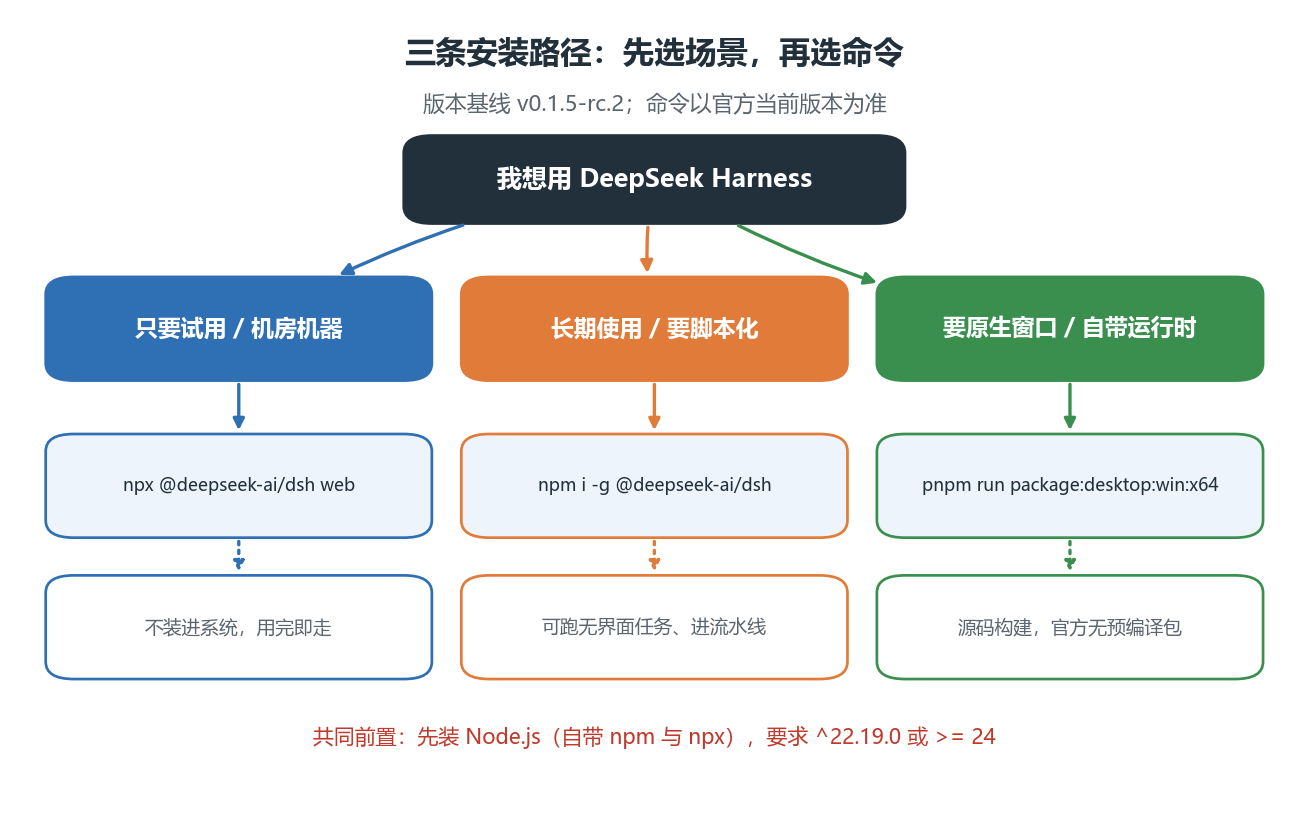
\includegraphics[keepaspectratio,alt={三条安装路径}]{figures/09-agent-basics/install_paths.png}}
\caption{三条安装路径}
\end{figure}

{\def\LTcaptype{none} % do not increment counter
\begin{longtable}[]{@{}
  >{\raggedright\arraybackslash}p{(\linewidth - 6\tabcolsep) * \real{0.2500}}
  >{\raggedright\arraybackslash}p{(\linewidth - 6\tabcolsep) * \real{0.2500}}
  >{\raggedright\arraybackslash}p{(\linewidth - 6\tabcolsep) * \real{0.2500}}
  >{\raggedright\arraybackslash}p{(\linewidth - 6\tabcolsep) * \real{0.2500}}@{}}
\toprule\noalign{}
\begin{minipage}[b]{\linewidth}\raggedright
路径
\end{minipage} & \begin{minipage}[b]{\linewidth}\raggedright
适合谁
\end{minipage} & \begin{minipage}[b]{\linewidth}\raggedright
需要准备
\end{minipage} & \begin{minipage}[b]{\linewidth}\raggedright
升级方式
\end{minipage} \\
\midrule\noalign{}
\endhead
\bottomrule\noalign{}
\endlastfoot
A 免安装 Web 版 & 第一次用、机房机器、不想改系统 & Node.js &
每次运行自动取最新（也可锁定版本） \\
B 全局 CLI 版 & 长期使用、要写脚本、要无界面跑任务 & Node.js + npm & npm
i -g @deepseek-ai/dsh@latest \\
C 桌面版 & 想要原生窗口与自带运行时 & Node.js + pnpm + 源码构建 &
重新拉源码构建 \\
\end{longtable}
}

共同前置只有一个：\textbf{Node.js}（npm 与 npx 随它一起安装，见 0.2 与
0.3）。官方仓库要求的版本是 \^{}22.19.0 或 \textgreater= 24.0.0。

\begin{Shaded}
\begin{Highlighting}[]
\ExtensionTok{node} \AttributeTok{{-}v}     \CommentTok{\# 例如 v24.19.0}
\ExtensionTok{npm} \AttributeTok{{-}v}      \CommentTok{\# 例如 11.x}
\end{Highlighting}
\end{Shaded}

如果 Node 版本过低，先升级：官网下载 LTS 版，或用 fnm / nvm
等版本管理器（第 0 章介绍过管理多个工具链的思路）。

\begin{quote}
提示：npm 下载慢时，可以临时用国内镜像（npm config set registry
https://registry.npmmirror.com）；企业网络或校园网如有代理，请按网络管理员要求配置。
\end{quote}

\subsection{2. 路径 A：免安装 Web
版（推荐先试）}\label{ux8defux5f84-aux514dux5b89ux88c5-web-ux7248ux63a8ux8350ux5148ux8bd5}

不安装任何全局命令，直接用 npx 拉起浏览器界面：

\begin{Shaded}
\begin{Highlighting}[]
\ExtensionTok{npx}\NormalTok{ @deepseek{-}ai/dsh web}
\end{Highlighting}
\end{Shaded}

会发生什么：

\begin{enumerate}
\def\labelenumi{\arabic{enumi}.}
\tightlist
\item
  首次运行会下载依赖包（视网络情况可能需要几分钟），请耐心等待；
\item
  服务默认在 http://127.0.0.1:3080 启动，本机运行时会自动打开浏览器；
\item
  \textbf{启动命令时所在的目录，就是默认工作区}，建议在一个专门的项目目录里执行；
\item
  关闭：回到终端按 Ctrl+C。
\end{enumerate}

常用参数：

\begin{Shaded}
\begin{Highlighting}[]
\ExtensionTok{npx}\NormalTok{ @deepseek{-}ai/dsh web }\AttributeTok{{-}{-}port}\NormalTok{ 8080    }\CommentTok{\# 换端口（被占用时很有用）}
\ExtensionTok{npx}\NormalTok{ @deepseek{-}ai/dsh web }\AttributeTok{{-}{-}no{-}open}      \CommentTok{\# 只启动服务，不开浏览器}
\ExtensionTok{npx}\NormalTok{ @deepseek{-}ai/dsh web }\AttributeTok{{-}{-}help}         \CommentTok{\# 查看当前版本支持的全部参数}
\end{Highlighting}
\end{Shaded}

\begin{quote}
说明：如果通过 SSH
在服务器上启动，终端只会打印地址，需要你在本地做端口转发（进阶用法，本节不展开）。
\end{quote}

\subsection{3. 路径 B：全局 CLI
版（长期使用）}\label{ux8defux5f84-bux5168ux5c40-cli-ux7248ux957fux671fux4f7fux7528}

装一次，长期用：

\begin{Shaded}
\begin{Highlighting}[]
\ExtensionTok{npm}\NormalTok{ i }\AttributeTok{{-}g}\NormalTok{ @deepseek{-}ai/dsh      }\CommentTok{\# 全局安装}
\ExtensionTok{dsh} \AttributeTok{{-}{-}version}                  \CommentTok{\# 确认版本}
\ExtensionTok{dsh}\NormalTok{ web                        }\CommentTok{\# 等价于 npx 的浏览器界面}
\end{Highlighting}
\end{Shaded}

本地版真正多出来的能力是\textbf{无界面（headless）任务}------让 Agent
跑完一件事直接打印结果，适合写进脚本：

\begin{Shaded}
\begin{Highlighting}[]
\ExtensionTok{dsh} \AttributeTok{{-}{-}profile}\NormalTok{ headless }\StringTok{"统计当前目录下所有 Python 文件的行数，输出一个表格"}
\end{Highlighting}
\end{Shaded}

其他自查入口：

\begin{Shaded}
\begin{Highlighting}[]
\ExtensionTok{dsh} \AttributeTok{{-}{-}help}                          \CommentTok{\# 启动器自身的参数}
\ExtensionTok{dsh}\NormalTok{ web }\AttributeTok{{-}{-}help}                      \CommentTok{\# Web 应用的参数}
\ExtensionTok{dsh} \AttributeTok{{-}{-}dump{-}config}                   \CommentTok{\# 查看合并后的配置树（不启动）}
\end{Highlighting}
\end{Shaded}

首次运行会在用户目录下创建配置与数据目录（Windows 为
C:/Users/你的用户名/.dsh，macOS 与 Linux 为
\textasciitilde/.dsh），里面包括设置、会话记录与凭据文件。\textbf{凭据文件不要提交到
git，也不要截图外发。}

升级与卸载：

\begin{Shaded}
\begin{Highlighting}[]
\ExtensionTok{npm}\NormalTok{ i }\AttributeTok{{-}g}\NormalTok{ @deepseek{-}ai/dsh@latest    }\CommentTok{\# 升级到最新}
\ExtensionTok{npm}\NormalTok{ rm }\AttributeTok{{-}g}\NormalTok{ @deepseek{-}ai/dsh          }\CommentTok{\# 卸载}
\end{Highlighting}
\end{Shaded}

{\def\LTcaptype{none} % do not increment counter
\begin{longtable}[]{@{}llll@{}}
\toprule\noalign{}
对比项 & npx 免安装 & 全局 CLI & headless \\
\midrule\noalign{}
\endhead
\bottomrule\noalign{}
\endlastfoot
是否改系统 & 否 & 是（全局包） & 是 \\
界面 & 浏览器 & 浏览器 & 无（打印结果） \\
适合 & 试用、机房 & 日常使用 & 批处理、自动化 \\
升级 & 每次运行自动解析 & 手动升级 & 跟随全局 \\
\end{longtable}
}

\subsection{4. 路径
C：桌面版（进阶，官方暂无预编译安装包）}\label{ux8defux5f84-cux684cux9762ux7248ux8fdbux9636ux5b98ux65b9ux6682ux65e0ux9884ux7f16ux8bd1ux5b89ux88c5ux5305}

先说结论：\textbf{官方目前没有发布桌面端安装包}，桌面端需要从源码构建，工程量偏大。课堂上了解它的定位与取舍即可，不要求真的构建。

桌面端是什么：它是完整 Web 应用外面的一层 Electron
壳------同一套界面与能力，多了原生窗口、菜单与系统通知，并\textbf{自带
Python / Node.js / pnpm
运行时}（对不想自己配环境的用户友好）。它默认使用 19387 端口，与 Web
版的 3080 分开。

源码构建（需要 Node 与 pnpm，命令以仓库当前版本为准）：

\begin{Shaded}
\begin{Highlighting}[]
\FunctionTok{git}\NormalTok{ clone https://github.com/deepseek{-}ai/deepseek{-}harness.git}
\BuiltInTok{cd}\NormalTok{ deepseek{-}harness}
\ExtensionTok{pnpm}\NormalTok{ install}
\ExtensionTok{pnpm}\NormalTok{ run build}
\ExtensionTok{pnpm}\NormalTok{ run package:desktop:win:x64        }\CommentTok{\# Windows}
\CommentTok{\#\# macOS Apple 芯片：pnpm run package:desktop:mac:arm64}
\CommentTok{\#\# macOS Intel：pnpm run package:desktop:mac:x64}
\end{Highlighting}
\end{Shaded}

只想先看看界面，可以用开发模式启动：pnpm run dev:desktop。

\begin{quote}
社区项目：有第三方开发者为 Windows 打包了桌面版分发（例如 GitHub 上的
DeepSeek-Harness-Desktop）。它\textbf{不是官方发布}，无法审计构建过程，安装前请自行评估供应链风险；课程不把它作为推荐路径。
\end{quote}

\subsection{5. 配置模型与 API
Key（重点）}\label{ux914dux7f6eux6a21ux578bux4e0e-api-keyux91cdux70b9}

\subsubsection{5.1 为什么需要 API
Key}\label{ux4e3aux4ec0ux4e48ux9700ux8981-api-key}

dsh
本身是免费开源软件，但它在运行时需要调用大模型，而模型调用按用量计费。因此你需要一个
DeepSeek 开放平台账号与 API Key------可以理解为''给 Agent 用的加油卡''。

\subsubsection{5.2 五步拿到 API
Key}\label{ux4e94ux6b65ux62ffux5230-api-key}

\begin{figure}
\centering
\pandocbounded{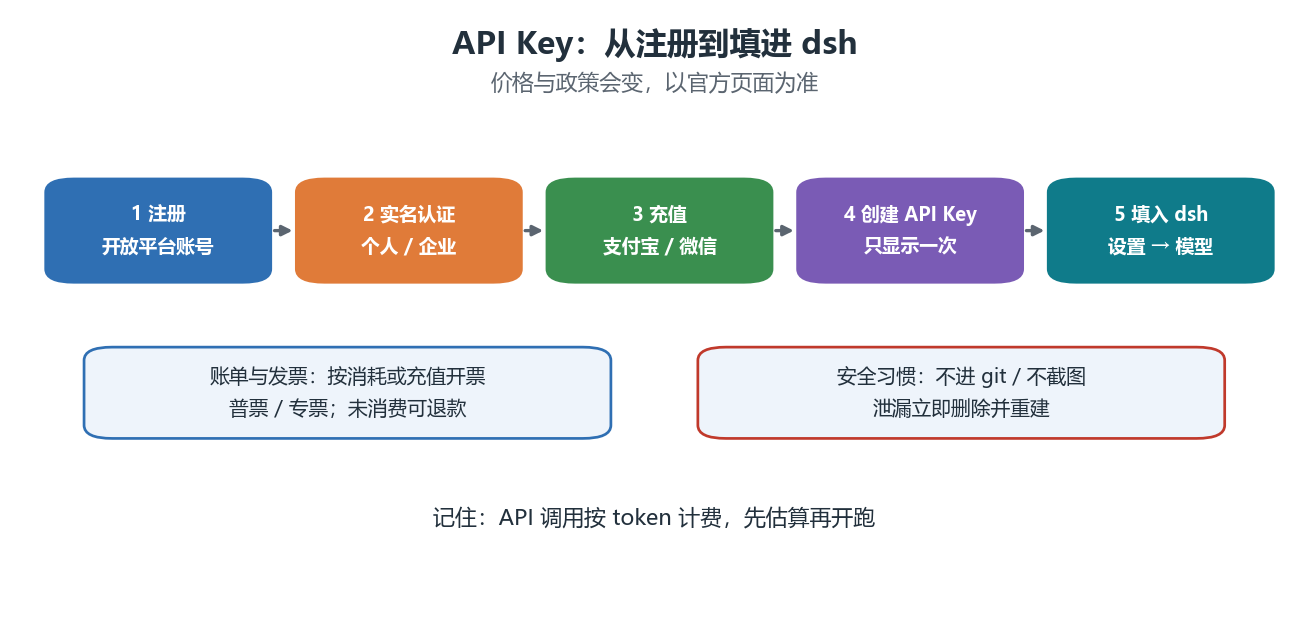
\includegraphics[keepaspectratio,alt={API Key 申请流程}]{figures/09-agent-basics/api_key_flow.png}}
\caption{API Key 申请流程}
\end{figure}

{\def\LTcaptype{none} % do not increment counter
\begin{longtable}[]{@{}
  >{\raggedright\arraybackslash}p{(\linewidth - 4\tabcolsep) * \real{0.3333}}
  >{\raggedright\arraybackslash}p{(\linewidth - 4\tabcolsep) * \real{0.3333}}
  >{\raggedright\arraybackslash}p{(\linewidth - 4\tabcolsep) * \real{0.3333}}@{}}
\toprule\noalign{}
\begin{minipage}[b]{\linewidth}\raggedright
步骤
\end{minipage} & \begin{minipage}[b]{\linewidth}\raggedright
在哪里做
\end{minipage} & \begin{minipage}[b]{\linewidth}\raggedright
关键细节
\end{minipage} \\
\midrule\noalign{}
\endhead
\bottomrule\noalign{}
\endlastfoot
1 注册 & platform.deepseek.com & 支持手机号 / 邮箱 / Google 登录 \\
2 实名认证 & 平台「实名认证」 &
分个人认证与企业认证；\textbf{决定后面发票抬头} \\
3 充值 & 平台「充值」页 & 支付宝 / 微信在线充值；对公汇款仅企业用户 \\
4 创建 API Key & 平台「API keys」页 & \textbf{Key
只显示一次}，当场复制保存 \\
5 填入 dsh & Web 界面「设置 → 模型 → DeepSeek」 & 粘贴 Key
并保存，立即生效，无需重启 \\
\end{longtable}
}

关于余额与发票（来自官方常见问题，2026-09 核对）：

\begin{itemize}
\tightlist
\item
  \textbf{充值余额永久有效}，未消费金额支持退款；
\item
  若同时存在赠送余额与充值余额，优先扣减赠送余额；
\item
  发票：在「账单 →
  发票管理」申请，可按\textbf{消耗金额}或\textbf{充值金额}开票；支持增值税普通发票与专用发票；个人认证可开个人或公司抬头，企业认证只能开企业认证主体的抬头；已开票金额需先作废才能退款。
\end{itemize}

\subsubsection{5.3 价格快照（2026-09-18
公布口径）}\label{ux4ef7ux683cux5febux71672026-09-18-ux516cux5e03ux53e3ux5f84}

价格以''每百万
tokens''计，且\textbf{分高峰与空闲两档}（空闲时段为高峰的一半）。

{\def\LTcaptype{none} % do not increment counter
\begin{longtable}[]{@{}
  >{\raggedright\arraybackslash}p{(\linewidth - 8\tabcolsep) * \real{0.2000}}
  >{\raggedright\arraybackslash}p{(\linewidth - 8\tabcolsep) * \real{0.2000}}
  >{\raggedright\arraybackslash}p{(\linewidth - 8\tabcolsep) * \real{0.2000}}
  >{\raggedright\arraybackslash}p{(\linewidth - 8\tabcolsep) * \real{0.2000}}
  >{\raggedright\arraybackslash}p{(\linewidth - 8\tabcolsep) * \real{0.2000}}@{}}
\toprule\noalign{}
\begin{minipage}[b]{\linewidth}\raggedright
模型
\end{minipage} & \begin{minipage}[b]{\linewidth}\raggedright
输入（缓存命中）
\end{minipage} & \begin{minipage}[b]{\linewidth}\raggedright
输入（未命中）
\end{minipage} & \begin{minipage}[b]{\linewidth}\raggedright
输出
\end{minipage} & \begin{minipage}[b]{\linewidth}\raggedright
备注
\end{minipage} \\
\midrule\noalign{}
\endhead
\bottomrule\noalign{}
\endlastfoot
deepseek-flash & 空闲 0.02 元 / 高峰 0.04 元 & 空闲 1 元 / 高峰 2 元 &
空闲 4 元 / 高峰 8 元 & 支持图片；上下文 1M \\
deepseek-v4-pro & 空闲 0.15 元 / 高峰 0.30 元 & 空闲 4.5 元 / 高峰 9.0
元 & 空闲 13.5 元 / 高峰 27.0 元 & 纯文本 \\
\end{longtable}
}

\begin{quote}
高峰时段：北京时间周一至周五
9:00--12:00、14:00--18:00；其余时间为空闲时段（半价）。价格与政策会调整，\textbf{以官方定价页为准}。
课程建议：练习与作业用 deepseek-flash；把重跑安排在空闲时段，能省一半。
\end{quote}

\subsubsection{5.4
估算一次任务花多少钱}\label{ux4f30ux7b97ux4e00ux6b21ux4efbux52a1ux82b1ux591aux5c11ux94b1}

下面这个脚本用一组''典型参数''估算费用：20K 未命中输入 + 60K 命中输入 +
15K 输出。

\begin{Shaded}
\begin{Highlighting}[]
\NormalTok{price }\OperatorTok{=}\NormalTok{ \{}\StringTok{"flash"}\NormalTok{: \{}\StringTok{"in\_miss"}\NormalTok{: }\FloatTok{1.0}\NormalTok{, }\StringTok{"in\_hit"}\NormalTok{: }\FloatTok{0.02}\NormalTok{, }\StringTok{"out"}\NormalTok{: }\FloatTok{4.0}\NormalTok{\},}
         \StringTok{"v4{-}pro"}\NormalTok{: \{}\StringTok{"in\_miss"}\NormalTok{: }\FloatTok{4.5}\NormalTok{, }\StringTok{"in\_hit"}\NormalTok{: }\FloatTok{0.15}\NormalTok{, }\StringTok{"out"}\NormalTok{: }\FloatTok{13.5}\NormalTok{\}\}}

\KeywordTok{def}\NormalTok{ cost(model, in\_miss\_k, in\_hit\_k, out\_k, peak}\OperatorTok{=}\VariableTok{False}\NormalTok{):}
\NormalTok{    p }\OperatorTok{=}\NormalTok{ price[model]}
\NormalTok{    factor }\OperatorTok{=} \FloatTok{2.0} \ControlFlowTok{if}\NormalTok{ peak }\ControlFlowTok{else} \FloatTok{1.0}
    \ControlFlowTok{return}\NormalTok{ factor }\OperatorTok{*}\NormalTok{ (p[}\StringTok{"in\_miss"}\NormalTok{] }\OperatorTok{*}\NormalTok{ in\_miss\_k }\OperatorTok{+}\NormalTok{ p[}\StringTok{"in\_hit"}\NormalTok{] }\OperatorTok{*}\NormalTok{ in\_hit\_k }\OperatorTok{+}\NormalTok{ p[}\StringTok{"out"}\NormalTok{] }\OperatorTok{*}\NormalTok{ out\_k) }\OperatorTok{/} \FloatTok{1000.0}

\BuiltInTok{print}\NormalTok{(}\StringTok{"flash  off{-}peak:"}\NormalTok{, }\BuiltInTok{round}\NormalTok{(cost(}\StringTok{"flash"}\NormalTok{, }\DecValTok{20}\NormalTok{, }\DecValTok{60}\NormalTok{, }\DecValTok{15}\NormalTok{), }\DecValTok{4}\NormalTok{), }\StringTok{"CNY"}\NormalTok{)}
\BuiltInTok{print}\NormalTok{(}\StringTok{"flash  peak    :"}\NormalTok{, }\BuiltInTok{round}\NormalTok{(cost(}\StringTok{"flash"}\NormalTok{, }\DecValTok{20}\NormalTok{, }\DecValTok{60}\NormalTok{, }\DecValTok{15}\NormalTok{, peak}\OperatorTok{=}\VariableTok{True}\NormalTok{), }\DecValTok{4}\NormalTok{), }\StringTok{"CNY"}\NormalTok{)}
\BuiltInTok{print}\NormalTok{(}\StringTok{"v4{-}pro off{-}peak:"}\NormalTok{, }\BuiltInTok{round}\NormalTok{(cost(}\StringTok{"v4{-}pro"}\NormalTok{, }\DecValTok{20}\NormalTok{, }\DecValTok{60}\NormalTok{, }\DecValTok{15}\NormalTok{), }\DecValTok{4}\NormalTok{), }\StringTok{"CNY"}\NormalTok{)}
\end{Highlighting}
\end{Shaded}

\begin{Shaded}
\begin{Highlighting}[]
\NormalTok{flash  off{-}peak: 0.0812 CNY}
\NormalTok{flash  peak    : 0.1624 CNY}
\NormalTok{v4{-}pro off{-}peak: 0.3015 CNY}
\end{Highlighting}
\end{Shaded}

结论：一次''读代码 + 改代码 + 跑测试 + 写说明''的中等任务，用
deepseek-flash 大约几分钱到几角钱；换成 deepseek-v4-pro 会贵 3 到 4 倍。

\subsection{6. 第一个任务（5
分钟验收）}\label{ux7b2cux4e00ux4e2aux4efbux52a15-ux5206ux949fux9a8cux6536}

\begin{enumerate}
\def\labelenumi{\arabic{enumi}.}
\tightlist
\item
  在浏览器界面点「选择工作区」，添加你的课程项目目录；
\item
  新建会话，把下面这段提示词发给它：
\end{enumerate}

\begin{Shaded}
\begin{Highlighting}[]
\NormalTok{请阅读当前工作区，回答三个问题：}
\NormalTok{1) 这个项目是做什么的？列出主要目录及用途；}
\NormalTok{2) 有哪些 Python 脚本？各自的作用是什么？}
\NormalTok{3) 如果我要新增一个数据分析脚本，应该放在哪里、遵循什么命名习惯？}
\NormalTok{只读不改：不要修改任何文件。}
\end{Highlighting}
\end{Shaded}

\begin{enumerate}
\def\labelenumi{\arabic{enumi}.}
\setcounter{enumi}{2}
\tightlist
\item
  观察它调用了哪些工具（读文件、列目录、搜索），以及它给出的结论有没有\textbf{证据}（引用了具体文件与行）。
\end{enumerate}

验收清单：

\begin{itemize}
\tightlist
\item
  它确实读了文件，而不是凭空描述；
\item
  它引用的文件名与目录结构能在你的项目里对上；
\item
  整个过程没有修改任何文件（因为你在提示词里要求了只读）。
\end{itemize}

\subsection{7. 常见故障排查}\label{ux5e38ux89c1ux6545ux969cux6392ux67e5}

{\def\LTcaptype{none} % do not increment counter
\begin{longtable}[]{@{}
  >{\raggedright\arraybackslash}p{(\linewidth - 4\tabcolsep) * \real{0.3333}}
  >{\raggedright\arraybackslash}p{(\linewidth - 4\tabcolsep) * \real{0.3333}}
  >{\raggedright\arraybackslash}p{(\linewidth - 4\tabcolsep) * \real{0.3333}}@{}}
\toprule\noalign{}
\begin{minipage}[b]{\linewidth}\raggedright
现象
\end{minipage} & \begin{minipage}[b]{\linewidth}\raggedright
可能原因
\end{minipage} & \begin{minipage}[b]{\linewidth}\raggedright
处理
\end{minipage} \\
\midrule\noalign{}
\endhead
\bottomrule\noalign{}
\endlastfoot
npm: command not found & 没装 Node.js & 安装 Node LTS 后重开终端 \\
npx 卡住不动 & 网络慢或代理 &
换网络、配置镜像或代理；耐心等待首次下载 \\
端口 3080 被占用 & 已有实例在跑 & 用 --port 8080
换端口，或先关闭旧实例 \\
浏览器打不开页面 & 服务没起来或防火墙拦截 &
看终端是否打印了地址、有没有报错 \\
输入框灰色不可用 & 没有选择工作区 & 先「选择工作区」并选中 \\
模型报鉴权错误 & Key 填错或已被删除 & 重新在「设置 → 模型」粘贴 Key \\
dsh 全局命令找不到 & 全局 bin 目录不在 PATH & 重开终端；或改回用 npx \\
PowerShell 执行策略报错 & 脚本被策略拦截 & 改用 npx
直接运行，或按学校要求调整策略 \\
任务跑很久没结果 & 任务过大或网络慢 & 缩小任务范围，先给最小复现 \\
\end{longtable}
}

\subsection{8.
升级与版本自查}\label{ux5347ux7ea7ux4e0eux7248ux672cux81eaux67e5}

\begin{Shaded}
\begin{Highlighting}[]
\ExtensionTok{npm}\NormalTok{ view @deepseek{-}ai/dsh dist{-}tags      }\CommentTok{\# 看官方最新}
\ExtensionTok{dsh} \AttributeTok{{-}{-}version}                            \CommentTok{\# 看本机版本}
\ExtensionTok{npm}\NormalTok{ i }\AttributeTok{{-}g}\NormalTok{ @deepseek{-}ai/dsh@latest         }\CommentTok{\# 升级}
\end{Highlighting}
\end{Shaded}

升级前建议读一眼 Releases
页的更新说明（官方每个版本都有中文条目），重点关注三类变化：\textbf{命令与参数}、\textbf{界面位置}、\textbf{模型名称}。这三类正是本节内容的来源。

\begin{quote}
本部分的维护机制：docs/build/dsh\_version.yaml
记录基线版本，docs/build/check\_dsh\_release.py
定期比对官方版本，双周自动提醒（见 docs/build/dsh\_更新SOP.md）。
\end{quote}

\subsection{本节小结}\label{ux672cux8282ux5c0fux7ed3-4}

\begin{enumerate}
\def\labelenumi{\arabic{enumi}.}
\tightlist
\item
  三条路径：npx 免安装（先试）、全局
  CLI（长期与脚本化）、桌面版（源码构建，进阶）。
\item
  共同前置是 Node.js（\^{}22.19.0 或 \textgreater= 24.0.0）。
\item
  API Key 五步：注册、实名、充值、创建、填入「设置 → 模型」。
\item
  计费按 token、分高峰与空闲；练习用 deepseek-flash，重跑放空闲时段。
\item
  Key 与凭据文件是资产：不进 git、不截图、泄漏立即删除重建。
\end{enumerate}

\subsection{思考题}\label{ux601dux8003ux9898-28}

\begin{enumerate}
\def\labelenumi{\arabic{enumi}.}
\tightlist
\item
  同学说''我用 npx 跑起来了，所以不用装 Node''------这句话哪里不对？
\item
  为什么教材不推荐学生用第三方打包的桌面版？请列出两条风险。
\item
  同样的任务，在高峰时段与空闲时段跑，费用差多少？请用 5.4
  的脚本算一个例子。
\item
  如果 API Key 不小心提交到了 git 仓库，你应该按什么顺序处理？
\item
  你想让 Agent 每天晚上自动跑一次数据检查，应该选哪条路径、用什么入口？
\end{enumerate}

\subsection{练习与延伸阅读}\label{ux7ec3ux4e60ux4e0eux5ef6ux4f38ux9605ux8bfb-1}

\begin{itemize}
\tightlist
\item
  练习：exercises/quiz.ipynb 第 5--6 题；
\item
  上机：lab/lab.ipynb Part A（环境自检，可无网络完成）；
\item
  参考：官方 README、Web UI 指南、模型配置指南（见 references.md）。
\end{itemize}

\newpage
